\chapter{Related Work}\label{sec:related}

Job scheduling with deadlines has been a well studied field.
In real-time systems, where each job has a hard deadline to be done,
Earliest Deadline First (EDF) policy has been widely adapted.
It is an optimal dynamic schedule policy on preemptive
uniprocessors~\cite{cite:pinedo2012scheduling}, which means if all
submit jobs in the system can be scheduled in a way that every job can
be done before deadline, EDF is able to schedule them so that all of
them can finish before their deadlines.

Various works studied dynamic scheduling methods for parallel real-time
jobs (PRJs) in clusters.
Qin et al. modeled parallel real-time jobs as directed acyclic graphs
and proposed a reliability-driven
method~\cite{cite:qin-reliability-driven}.
He et al. represented real-time processing as hybrid execution of
existing periodic jobs and newly arriving aperiodic jobs, and proposed a
scheduling method by modeling spare capabilities of new arriving
aperiodic parallel real-time jobs~\cite{cite:he-spare-capabilities}.
Xie et al. proposed TAPADS, Task Allocation for Parallel Applications
with Deadline and Security Constraints, which takes security constraints
into consideration~\cite{cite:xie-TAPADS,cite:xie2008security}.
In these cases, deadlines are hard.
If the system cannot guarantee a submitted job can be finished before
required deadline, it is thus rejected.

On the other hand, several works focused on scheduling with soft
deadlines, where missing deadlines is possible but might yield different
kind of costs.
Soft deadlines are also viewed as a kind of service level agreements
(SLAs) or Quality of Service (QoS) demands.
Service level agreements are usually applied in clusters that provide
charged computation services, so lots of works took user utility as
their objective.
For instance, Libra is a computational economy driven scheduling system
designed to support allocation of resources based on the users' quality
of service requirements~\cite{cite:libra}, and Yeo et al. used a linear
penalty model on user utility~\cite{cite:yeo-SLA-penalty}.
Also, job with QoS demands are often associated with grid computing; He
et al. proposed a two-level optimization --- MUSCLE, a multi-cluster
level scheduler, and TITAN, a single-cluster level workload manager ---
for scheduling in parallel jobs in multi-clusters and
grids~\cite{cite:he-muscle-titan}

Java Parallel Processing Framework (JPPF)~\cite{cite:JPPF} is a very
popular open-source job dispatching framework.
It has gained enormous amount of users with abundant customization APIs
, user friendly management tool in GUI
(figure~\ref{fig:jppf-management-tool}) and being extremely easy to
deploy.
However, because its design is to let available nodes pull tasks from a
queue, it is very hard to achieve node-aware scheduling that can assign
tasks to a certain machine explicitly.
\begin{figure}[htpb]
  \centering
  \resizebox{\linewidth}{!}{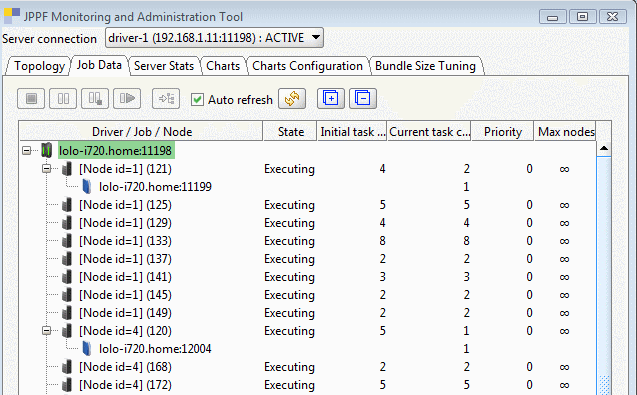
\includegraphics{figures/jppf.png}}
  \caption{Graphical Management Tool of JPPF}
  \label{fig:jppf-management-tool}
\end{figure}
